\newpage
\section{Conjuntos de entrenamiento}

\subsection{CROHME}

El conjunto de datos de entrenamiento para el desarrollo de la red es el denominado \textbf{CROHME} por sus siglas en inglés: \textbf{Competition on Recognition of Online Handwritten Mathematical Expressions} publicado por los organizadores de la competencia internacional CROHME; para el caso del conjunto de entrenamiento fue posible reunir 7169 elementos que de acuerdo a investigación previa \cite{chino}, son relativamente pocos  para esperar una buena precisión, los  elementos en en el conjunto son archivos de tipo INKML.
\subsubsection{Formato del conjunto de datos}

Como ya se mencionó, los elementos del conjunto son archivos de tipo INKML (Ink Markup Language) y que principalmente se compone de tres partes:

\begin{itemize}
	\item Ink: Un conjunto de trazos definidos por puntos.
	\item Nivel de símbolo Ground-Truth: La segmentación e información de etiqueta de cada símbolo de la expresión.
	\item Ground-truth: La estructura MATHML de la expresión.
\end{itemize}

La información de \textit{Ground-Truth} tanto de nivel de símbolo como de la expresión matemática fueron ingresadas manualmente por los colaboradores de la generación del conjunto, además, alguna información general es agregada en el archivo:

\begin{itemize}
	\item Los canales (en este caso X, Y)
	\item La información del escritor (Identificación, entrega, edad, Mano dominante, género, etc ), si está disponible.
	\item Ground-Truth en \LaTeX{} para fácilmente renderizarlo.
\end{itemize} 

Es importante señalar que al pasar los archivos de INKML a imagen PNG, se obtuvieron imágenes de diferentes tamaños, sin embargo en el entrenamiento las imágenes que se utilizaron fueron de 300x150 px.

A continuación se muestra un ejemplo de un archivo del dataset que representa la expresión \$2 \^\ \{-1 \} \$:\\
 $2^{-1}$ renderizado.
\lstinputlisting[language=XML]{capitulo5/dataset/Inkdata_temp_InkFR_HPR_EQU_NOC_scc696_fi6_db144195.inkml}
Sin embargo, para el propósito del trabajo terminal, el conjunto de datos no es útil en este formato, por lo que se tenía que transformar la información de los trazos en imágenes.
\subsubsection{Conversión a imagen}
Con la información que contiene el archivo INKML es posible generar una imagen con los puntos de los trazos en negro y fondo blanco. El primer reto fue identificar las etiquetas que contenían a los trazos, para ello se utilizó la biblioteca de Python xml.etree y una función de terceros para poder utilizar dichos trazos posteriormente:

\lstinputlisting[language=Python]{capitulo5/dataset/getTraces.py}

Una vez obtenidos los trazos y con ayuda de matplotlib fueron separados como puntos $x,y$ y utilizados en la función plot de matplotlib para posteriormente guardarlo como imagen.

\lstinputlisting[language=Python]{capitulo5/dataset/inkml2img_short.py}

Este procedimiento tenía que realizarse por cada uno de los elementos del conjunto de entrenamiento, además de también extraer la expresión matemática encerrada entre las etiquetas \textbf{$<$annotation$>$$<$/annotation$>$} con el atributo \textbf{type}, para ello nuevamente se utilizó la biblioteca de python xml.etree para acceder a los nodos del árbol directamente:
\lstinputlisting[language=Python]{capitulo5/dataset/tag.py}
Con estos subscripts fue posible desarrollar una biblioteca que permite acceder a la carpeta con el conjunto de entrenamiento en formato inkml y guardarlos como imagen en otra carpeta junto con un archivo CSV conteniendo la ruta relativa de la imagen y la expresión en \LaTeX{} correspondiente separados por coma.

\lstinputlisting[language=Python, firstline = 1, lastline=10]{capitulo5/dataset/training.csv}
\subsubsection{Generador de secuencia de tokens}
El archivo CSV generado con lo descrito anteriormente no es suficiente para cargarlo en TensorFlow, la expresión matemática en \LaTeX{} debía ser expresada como una secuencia numérica, por lo que se necesitaba identificar a cada símbolo con un número único y conformar a la secuencia, de modo que la estructura del archivo CSV pasaría de tener la forma \textbf{RUTA\_IMAGEN}, \textbf{EXPRESION\_LATEX} a tener la forma \textbf{RUTA\_IMAGEN}, \textbf{SECUENCIA\_NUMÉRICA}, teniendo así una nueva representación del conjunto de entrenamiento conformada por una carpeta con las imágenes y un archivo CSV previamente descrito para poder cargarse en TensorFlow.

Para esto, se desarrolló gracias a lex en Python un script para especificar los tokens tomando como base los símbolos especificados en la sección \ref{sec:del_exp}.\\\\
\lstinputlisting[language=Python, lastline=10]{capitulo5/dataset/Rules.py}

\lstinputlisting[language=Python, firstline = 26, lastline=44]{capitulo5/dataset/Analyzer.py}

\lstinputlisting[firstline = 1, lastline=10]{capitulo5/dataset/tokenized_training.csv}

\vspace{1em}
Es importante destacar que se debe también guardar este mapeo único y no alterar el orden, por lo que de requerir agregar nuevos símbolos al conjunto es necesario hacerlo al final de los ya existentes, ya que la red entrenada devuelve secuencias numéricas que deben mapearse para tener la correspondiente expresión en \LaTeX{}.

\subsection{Harvard 100k}

El segundo conjunto de entrenamiento utilizado fue el provisto por \cite{harvard}. Los investigadores que realizaron el paper liberaron el conjunto de entrenamiento que recabaron, el cual cuenta con alrededor de cien mil expresiones matemáticas escritas a computadora.

Este conjunto de entrenamiento puede descargarse libremente en la página provista por el artículo. Consiste en un conjunto de imágenes png sin preprocesar y sus respectivos resultados esperados (Grounth-Truth). Así mismo, los autores del artículo proveen scripts de normalización y de preprocesado para el tratamiento de las imágenes. Estos scripts se pueden encontrar en el github del artículo \cite{harvard-scripts}.

Se procedio a preprocesar las imágenes con los scripts provistos por los investigadores de Harvard y se obtuvo un conjunto de entrenamiento con 78000 imágenes. Debido a que en el presente Trabajo Terminal las estructuras matriciales no estan contempladas, se descartaron todas las imágenes que contuvieran matrices, arreglos o listas, así como aquellas que produjeron errores tras ser procesadas. El conjunto final contiene 73000 imágenes de distintos tamaños los cuales son: (200,50), (240,40), (280,40), (360,60), (160,40), (360,50), (120,50), (320,50), (400,50), (360,10), (360,40), (200,40), (320,40), (280,50) y (240,50). En la Figura \ref{fig:harvard-example} se puede ver un ejemplo de una imagen del conjunto de entrenamiento de Harvard.

\begin{figure}[H]
	\centering
	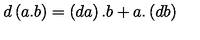
\includegraphics{capitulo5/dataset/harvard}
	\caption{Ejemplo de una imagen del conjunto de entrenamiento Harvard 100k}
	\label{fig:harvard-example}
\end{figure}

\subsection{Normalización}

Entre los scripts provistos por los investigadores de Harvard \cite{harvard-scripts}, se encuentra un normalizador. Este código, realiza una serie de transformaciones seguras con el fin de estandarizar ciertas inconsitencias con las expresiones en \LaTeX{}. Un ejemplo podría ser las distintas formas que se tienen para expresar un exponente: \textit{a \^\ b} y \textit{a \^\ \{ b \}} producirían el mismo resultado. Para mejorar el rendimiento de la red, ambos conjuntos de entrenamiento fueron preprocesados con el script de normalizado.

Cabe mencionar que ambos conjuntos de entrenamiento fueron unificados mediante la combinación de su Grounth-Truth, por lo que es posible utilizarlos indistintamente. Para unificarlos se proceso el conjunto CROHME para convertir sus tokens en tokens del conjunto de Harvard. El código usado se muestra a continuación.

\lstinputlisting[language=Python]{capitulo5/dataset/converter.py}

\newpage


